\tikzset{every picture/.style={line width=0.75pt}} %set default line width to 0.75pt        

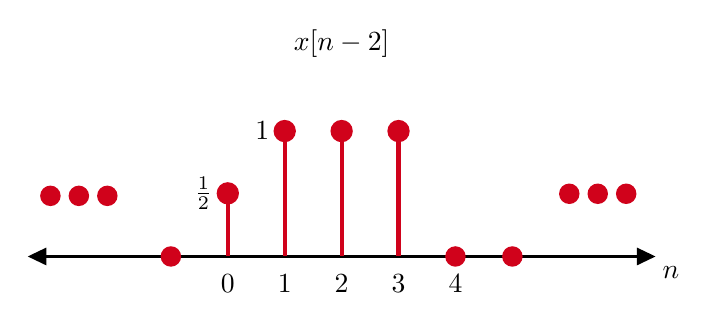
\begin{tikzpicture}[x=0.75pt,y=0.75pt,yscale=-1,xscale=1]
%uncomment if require: \path (0,437); %set diagram left start at 0, and has height of 437

%Straight Lines [id:da6728625031917905] 
\draw    (437.71,170) -- (141.29,170) ;
\draw [shift={(138.29,170)}, rotate = 360] [fill={rgb, 255:red, 0; green, 0; blue, 0 }  ][line width=0.08]  [draw opacity=0] (8.93,-4.29) -- (0,0) -- (8.93,4.29) -- cycle    ;
\draw [shift={(440.71,170)}, rotate = 180] [fill={rgb, 255:red, 0; green, 0; blue, 0 }  ][line width=0.08]  [draw opacity=0] (8.93,-4.29) -- (0,0) -- (8.93,4.29) -- cycle    ;
%Straight Lines [id:da7446362084910108] 
\draw [color={rgb, 255:red, 208; green, 2; blue, 27 }  ,draw opacity=1 ][fill={rgb, 255:red, 208; green, 2; blue, 27 }  ,fill opacity=1 ][line width=1.5]    (289.5,109.58) -- (289.5,170) ;
\draw [shift={(289.5,109.58)}, rotate = 90] [color={rgb, 255:red, 208; green, 2; blue, 27 }  ,draw opacity=1 ][fill={rgb, 255:red, 208; green, 2; blue, 27 }  ,fill opacity=1 ][line width=1.5]      (0, 0) circle [x radius= 4.36, y radius= 4.36]   ;
%Straight Lines [id:da5436064593523208] 
\draw [color={rgb, 255:red, 208; green, 2; blue, 27 }  ,draw opacity=1 ][fill={rgb, 255:red, 208; green, 2; blue, 27 }  ,fill opacity=1 ][line width=1.5]    (316.92,109.58) -- (316.92,170) ;
\draw [shift={(316.92,109.58)}, rotate = 90] [color={rgb, 255:red, 208; green, 2; blue, 27 }  ,draw opacity=1 ][fill={rgb, 255:red, 208; green, 2; blue, 27 }  ,fill opacity=1 ][line width=1.5]      (0, 0) circle [x radius= 4.36, y radius= 4.36]   ;
%Straight Lines [id:da6606279801735465] 
\draw [color={rgb, 255:red, 208; green, 2; blue, 27 }  ,draw opacity=1 ][fill={rgb, 255:red, 208; green, 2; blue, 27 }  ,fill opacity=1 ][line width=1.5]    (262.08,109.58) -- (262.08,170) ;
\draw [shift={(262.08,109.58)}, rotate = 90] [color={rgb, 255:red, 208; green, 2; blue, 27 }  ,draw opacity=1 ][fill={rgb, 255:red, 208; green, 2; blue, 27 }  ,fill opacity=1 ][line width=1.5]      (0, 0) circle [x radius= 4.36, y radius= 4.36]   ;
%Straight Lines [id:da11638977872575196] 
\draw [color={rgb, 255:red, 208; green, 2; blue, 27 }  ,draw opacity=1 ][fill={rgb, 255:red, 208; green, 2; blue, 27 }  ,fill opacity=1 ][line width=1.5]    (234.66,139.58) -- (234.66,170) ;
\draw [shift={(234.66,139.58)}, rotate = 90] [color={rgb, 255:red, 208; green, 2; blue, 27 }  ,draw opacity=1 ][fill={rgb, 255:red, 208; green, 2; blue, 27 }  ,fill opacity=1 ][line width=1.5]      (0, 0) circle [x radius= 4.36, y radius= 4.36]   ;
%Shape: Circle [id:dp16680741947391897] 
\draw  [color={rgb, 255:red, 208; green, 2; blue, 27 }  ,draw opacity=1 ][fill={rgb, 255:red, 208; green, 2; blue, 27 }  ,fill opacity=1 ] (202.81,170) .. controls (202.81,167.56) and (204.79,165.58) .. (207.24,165.58) .. controls (209.68,165.58) and (211.66,167.56) .. (211.66,170) .. controls (211.66,172.44) and (209.68,174.42) .. (207.24,174.42) .. controls (204.79,174.42) and (202.81,172.44) .. (202.81,170) -- cycle ;
%Shape: Circle [id:dp24325412264442625] 
\draw  [color={rgb, 255:red, 208; green, 2; blue, 27 }  ,draw opacity=1 ][fill={rgb, 255:red, 208; green, 2; blue, 27 }  ,fill opacity=1 ] (367.34,170) .. controls (367.34,167.56) and (369.32,165.58) .. (371.76,165.58) .. controls (374.21,165.58) and (376.19,167.56) .. (376.19,170) .. controls (376.19,172.44) and (374.21,174.42) .. (371.76,174.42) .. controls (369.32,174.42) and (367.34,172.44) .. (367.34,170) -- cycle ;
%Shape: Circle [id:dp3570850369681069] 
\draw  [color={rgb, 255:red, 208; green, 2; blue, 27 }  ,draw opacity=1 ][fill={rgb, 255:red, 208; green, 2; blue, 27 }  ,fill opacity=1 ] (394.76,139.79) .. controls (394.76,137.35) and (396.74,135.37) .. (399.19,135.37) .. controls (401.63,135.37) and (403.61,137.35) .. (403.61,139.79) .. controls (403.61,142.23) and (401.63,144.21) .. (399.19,144.21) .. controls (396.74,144.21) and (394.76,142.23) .. (394.76,139.79) -- cycle ;
%Shape: Circle [id:dp3297830684019689] 
\draw  [color={rgb, 255:red, 208; green, 2; blue, 27 }  ,draw opacity=1 ][fill={rgb, 255:red, 208; green, 2; blue, 27 }  ,fill opacity=1 ] (408.47,139.79) .. controls (408.47,137.35) and (410.45,135.37) .. (412.9,135.37) .. controls (415.34,135.37) and (417.32,137.35) .. (417.32,139.79) .. controls (417.32,142.23) and (415.34,144.21) .. (412.9,144.21) .. controls (410.45,144.21) and (408.47,142.23) .. (408.47,139.79) -- cycle ;
%Shape: Circle [id:dp12503088297139797] 
\draw  [color={rgb, 255:red, 208; green, 2; blue, 27 }  ,draw opacity=1 ][fill={rgb, 255:red, 208; green, 2; blue, 27 }  ,fill opacity=1 ] (422.19,139.79) .. controls (422.19,137.35) and (424.16,135.37) .. (426.61,135.37) .. controls (429.05,135.37) and (431.03,137.35) .. (431.03,139.79) .. controls (431.03,142.23) and (429.05,144.21) .. (426.61,144.21) .. controls (424.16,144.21) and (422.19,142.23) .. (422.19,139.79) -- cycle ;
%Shape: Circle [id:dp7532419367276733] 
\draw  [color={rgb, 255:red, 208; green, 2; blue, 27 }  ,draw opacity=1 ][fill={rgb, 255:red, 208; green, 2; blue, 27 }  ,fill opacity=1 ] (144.76,140.79) .. controls (144.76,138.35) and (146.74,136.37) .. (149.19,136.37) .. controls (151.63,136.37) and (153.61,138.35) .. (153.61,140.79) .. controls (153.61,143.23) and (151.63,145.21) .. (149.19,145.21) .. controls (146.74,145.21) and (144.76,143.23) .. (144.76,140.79) -- cycle ;
%Shape: Circle [id:dp8234155158894582] 
\draw  [color={rgb, 255:red, 208; green, 2; blue, 27 }  ,draw opacity=1 ][fill={rgb, 255:red, 208; green, 2; blue, 27 }  ,fill opacity=1 ] (158.47,140.79) .. controls (158.47,138.35) and (160.45,136.37) .. (162.9,136.37) .. controls (165.34,136.37) and (167.32,138.35) .. (167.32,140.79) .. controls (167.32,143.23) and (165.34,145.21) .. (162.9,145.21) .. controls (160.45,145.21) and (158.47,143.23) .. (158.47,140.79) -- cycle ;
%Shape: Circle [id:dp3922736373189596] 
\draw  [color={rgb, 255:red, 208; green, 2; blue, 27 }  ,draw opacity=1 ][fill={rgb, 255:red, 208; green, 2; blue, 27 }  ,fill opacity=1 ] (172.19,140.79) .. controls (172.19,138.35) and (174.16,136.37) .. (176.61,136.37) .. controls (179.05,136.37) and (181.03,138.35) .. (181.03,140.79) .. controls (181.03,143.23) and (179.05,145.21) .. (176.61,145.21) .. controls (174.16,145.21) and (172.19,143.23) .. (172.19,140.79) -- cycle ;
%Shape: Circle [id:dp08799827139095029] 
\draw  [color={rgb, 255:red, 208; green, 2; blue, 27 }  ,draw opacity=1 ][fill={rgb, 255:red, 208; green, 2; blue, 27 }  ,fill opacity=1 ] (339.92,170) .. controls (339.92,167.56) and (341.9,165.58) .. (344.34,165.58) .. controls (346.78,165.58) and (348.76,167.56) .. (348.76,170) .. controls (348.76,172.44) and (346.78,174.42) .. (344.34,174.42) .. controls (341.9,174.42) and (339.92,172.44) .. (339.92,170) -- cycle ;

% Text Node
\draw (442.71,173.4) node [anchor=north west][inner sep=0.75pt]    {$n$};
% Text Node
\draw (289.5,75.6) node [anchor=south] [inner sep=0.75pt]    {$x[ n-2]$};
% Text Node
\draw (234.66,177.4) node [anchor=north] [inner sep=0.75pt]    {$0$};
% Text Node
\draw (262.08,177.4) node [anchor=north] [inner sep=0.75pt]    {$1$};
% Text Node
\draw (289.5,177.4) node [anchor=north] [inner sep=0.75pt]    {$2$};
% Text Node
\draw (316.92,177.4) node [anchor=north] [inner sep=0.75pt]    {$3$};
% Text Node
\draw (344.34,177.4) node [anchor=north] [inner sep=0.75pt]    {$4$};
% Text Node
\draw (228.66,139.58) node [anchor=east] [inner sep=0.75pt]    {$\frac{1}{2}$};
% Text Node
\draw (256.08,109.58) node [anchor=east] [inner sep=0.75pt]    {$1$};


\end{tikzpicture}
